\section{Overview of the concurrency in \Kotlin and \Go}

As specified in the introduction, \Kotlin and \Go exposes concurrency thanks to \textbf{coroutines} and other tools that let the developer manage their synchronization.

As we already said, coroutines are lightweight processes for cooperation that executes on OS threads and that can suspend at a certain point and later resumed at the same point but with the possibility to execute on a different thread. The main advantage by using coroutines instead threads is that switching between then does not require any \textit{system call} ensuring lower management costs.
This introduces great advantages especially for \textit{asynchronous} computation.

\subsection{\Kotlin concurrency overview}

We said that \Kotlin is based on the \texttt{JVM} (but can also compile \texttt{JavaScript} or native using \href{https://llvm.org/}{LLVM}) and is interoperable with \texttt{Java}. The main implementation of \Kotlin is done in its compiler: for \Kotlin on \texttt{JVM}, all classes are compiled as normal \texttt{Java} classes. This means that \textbf{\Kotlin can access to all \texttt{threading}} packages exposed by \texttt{Java} (and this is also valid for \texttt{Android}). So, in \Kotlin \textbf{it is possible to use the standard threads} that are provided by \texttt{Java}.

Even if there is the possibility to use the standard \texttt{Java} threads, as anticipated, \Kotlin introduces the new \href{https://github.com/Kotlin/kotlinx.coroutines}{\texttt{kotlinx.coroutines}} library for realizing concurrency by adopting \textit{coroutines}. Coroutines are \textit{instances of suspendable computation} that let the developer to easily write \textbf{asynchronous and non-blocking code} that can run concurrently, without using \textit{callback} or \textit{promises}.
The main mechanism in which \Kotlin coroutines are based is the \textbf{suspending function}: special \Kotlin method that can suspend the execution of the current coroutine without blocking the current thread.

\subsubsection{Realization of coroutines in \Kotlin}

To go into the details of the coroutine in \Kotlin, we have to introduce some basic concepts\footnote{See \href{https://medium.com/mobile-app-development-publication/kotlin-coroutine-scope-context-and-job-made-simple-5adf89fcfe94}{medium.com} for additional details.}:
\begin{itemize}
	\item \href{https://kotlinlang.org/api/kotlinx.coroutines/kotlinx-coroutines-core/kotlinx.coroutines/-job/}{\underline{\textbf{\textcolor{ForestGreen}{Job}}}}:\\
	The object that represents a \textit{background job} of a coroutine. When a coroutine is launched, the \href{https://kotlinlang.org/api/kotlinx.coroutines/kotlinx-coroutines-core/kotlinx.coroutines/launch.html}{\texttt{launch}} method immediately returns the reference to the \texttt{Job} associated to the coroutine. \textbf{A job represents the lifecycle of a coroutine} and can be used to \textit{cancel} its execution. Then, it can have six possible states, each coded by a combination of the three properties of the \texttt{Job} class: \href{https://kotlinlang.org/api/kotlinx.coroutines/kotlinx-coroutines-core/kotlinx.coroutines/-job/is-active.html}{\texttt{isActive}}, \href{https://kotlinlang.org/api/kotlinx.coroutines/kotlinx-coroutines-core/kotlinx.coroutines/-job/is-completed.html}{\texttt{isCompleted}} and \href{https://kotlinlang.org/api/kotlinx.coroutines/kotlinx-coroutines-core/kotlinx.coroutines/-job/is-cancelled.html}{\texttt{isCancelled}}.
	This table summarizes the possible states of a \texttt{Job} and the value of the three properties for each state:
	\begin{table}[h!]
		\centering
		\begin{tabular}{ccccc}
			\textbf{State} & \textbf{Type} & \textbf{isActive} & \textbf{isCompleted} & \textbf{isCancelled} \\
			\textit{New}        & initial   & \texttt{false} & \texttt{false} & \texttt{false} \\
			\textit{Active}     & initial   & \texttt{true}  & \texttt{false} & \texttt{false} \\
			\textit{Completing} & transient & \texttt{true}  & \texttt{false} & \texttt{false} \\
			\textit{Cancelling} & transient & \texttt{false} & \texttt{false} & \texttt{true}  \\
			\textit{Cancelled}  & final     & \texttt{false} & \texttt{true}  & \texttt{true}  \\
			\textit{Completed}  & final     & \texttt{false} & \texttt{true}  & \texttt{false}
		\end{tabular}
		\caption{States of a \texttt{Job}}
		\label{tab:job_states}
	\end{table}

	\begin{figure}[h!]
		\centering
		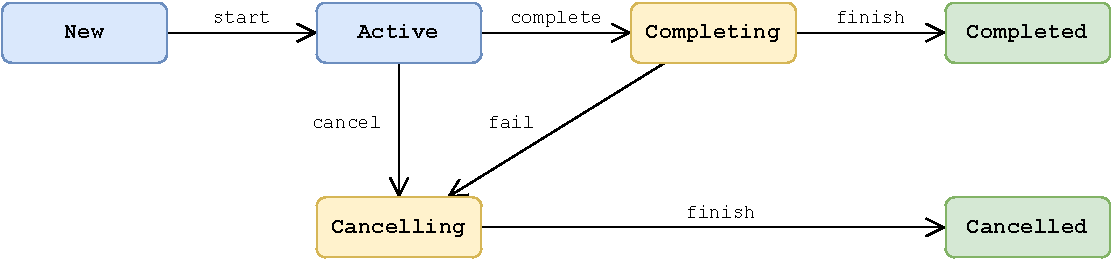
\includegraphics[width=0.9\textwidth]{img/kotlin_coroutines_lifecycle}
		\caption{Lifecycle of \Kotlin coroutine in \texttt{Job}}
		\label{fig::kotlin_coroutines_lifecycle}
	\end{figure}

	The figure \ref{fig::kotlin_coroutines_lifecycle} represents the entire lifecycle of a \texttt{Job}, so it also represents the lifecycle of a \Kotlin coroutine.
	
	\item \href{https://kotlinlang.org/api/kotlinx.coroutines/kotlinx-coroutines-core/kotlinx.coroutines/-coroutine-dispatcher/}{\underline{\textbf{\textcolor{ForestGreen}{CoroutineDispatcher}}}}:\\
	As we already said, in their lifecycle coroutine can run in different threads. For example, suppose to have a coroutine $C_1$ that is started on the thread $T_1$ that executes its code:
	\begin{enumerate}
		\item $C_1$ starts its execution on thread $T_1$;
		\item during its execution, $C_1$ encounter an instruction $I_1$ that suspends it waiting for something;
		\item $C_1$ is suspended by $I_1$ and another coroutine $C_2$ starts to execute on $T_1$;
		\item $C_2$ is executing on $T_1$ while $I_1$ returns resuming $C_1$ from its suspension, but now $T_1$ is not available because it is executing the code of $C_2$;
		\item $C_1$ may execute on another available thread $T_2$ while $C_2$ continue to run in parallel on $T_1$ (if the configuration allows it).
	\end{enumerate}
	\textbf{\texttt{CoroutineDispatcher} is the object that \textit{dispatch} the coroutine between the different available threads}. The \texttt{CoroutineDispatcher} is important because it determines in which thread a couroutine can run: for example, in \texttt{Android} using \href{https://kotlinlang.org/api/kotlinx.coroutines/kotlinx-coroutines-core/kotlinx.coroutines/-dispatchers/-main.html}{Dispatchers.Main} means that the coroutine will be executed confined to the \texttt{Main} thread\footnote{In this case, the coroutine can update the \texttt{UI}. There are also dispatchers for \texttt{JavaFX} or \texttt{Swing} for \texttt{Kotlin JVM} to force coroutines to be executed on the thread that can update the user interface.}.
	
	By default, when a coroutine is created, it is used the \href{https://kotlinlang.org/api/kotlinx.coroutines/kotlinx-coroutines-core/kotlinx.coroutines/-dispatchers/-default.html}{\texttt{Dispatchers.Default}} that uses \textit{worker} threads, a shared pool of threads on \texttt{JVM} in which coroutines can execute in parallel. 
	
	\item \href{https://kotlinlang.org/api/latest/jvm/stdlib/kotlin.coroutines/-coroutine-context/}{\underline{\textbf{\textcolor{ForestGreen}{CoroutineContext}}}}:\\
	Each coroutine in \Kotlin has a \textit{context} that is \textit{immutable}. A context is simply a set of \textit{elements} that realizes the concept of \textit{context} in which the coroutine executes.
	The main elements in a context are:
	\begin{itemize}
		\item the \texttt{Job} that represents the coroutine;
		\item the \texttt{CoroutineDispatcher} that dispatches the execution of coroutine over the threads;
		\item the \texttt{CoroutineName} that is the name associated to the coroutine (useful for debugging);
		\item the \texttt{CoroutineExceptionHandler} that is an handler for all the exception thrown during the execution of the coroutine;
		\item the \texttt{ContinuationInterceptor} that allows to define \textit{how} the coroutine should continue after a resume (a sort of \textit{callback} that is invoked on coroutine resume).
	\end{itemize}
	
	Notice that \textbf{\texttt{CoroutineContext} is immutable, but it is possible to add elements using the plus operator} that produces a new context instance. In addition, \textbf{all of these elements extends \texttt{CoroutineContext}} so, using \href{https://kotlinlang.org/api/latest/jvm/stdlib/kotlin.coroutines/-coroutine-context/plus.html}{\texttt{plus}} operator let to easily create a context that is a \textit{join} of the other.
	For example:
	\begin{lstlisting}[language=Kotlin,numbers=none]
		val newContext = CoroutineName("MyCoroutine") + Dispatchers.Main
	\end{lstlisting}
	creates a new context named \textit{MyCoroutine} in which coroutine will be executed using \texttt{Disparchers.Main}.
	
	\textbf{A context can be passed to the coroutine builder before launching it or, if the context has to be changed while coroutine is running, it is possible to use \href{https://kotlinlang.org/api/kotlinx.coroutines/kotlinx-coroutines-core/kotlinx.coroutines/with-context.html}{withContext} suspend function}.
	\Kotlin has also a default context for builders that is \href{https://kotlinlang.org/api/latest/jvm/stdlib/kotlin.coroutines/-empty-coroutine-context/}{\texttt{EmptyCoroutineContext}} which can be also used with \texttt{plus} operator to create new contexts.
	
	\item \href{https://kotlinlang.org/api/kotlinx.coroutines/kotlinx-coroutines-core/kotlinx.coroutines/-coroutine-scope/}{\underline{\textbf{\textcolor{ForestGreen}{CoroutineScope}}}}:\\
	Each coroutine in \Kotlin must have a \textit{scope} which delimits the lifetime of the coroutine. The \texttt{CoroutineScope} consists in only one property: \texttt{coroutineContext}, an instance of \texttt{CoroutineContext}.
	In addition to this, the \texttt{CoroutineScope} has also some \href{https://kotlinlang.org/docs/extensions.html}{\textit{extension functions}} such as \href{https://kotlinlang.org/api/kotlinx.coroutines/kotlinx-coroutines-core/kotlinx.coroutines/launch.html}{\texttt{launch}} that is a builder for coroutines.
	
	Then, when \texttt{launch} is invoked using a \texttt{CoroutineScope}, the function launches a new coroutine and its context is \textit{inherited} from those of the scope.
	In this way, all the elements of the parents and its cancellation are propagated to the child; then, if a scope is cancelled, all the coroutine launched starting from it will be cancelled.
\end{itemize}

\begin{center}
	In \Kotlin \textbf{the concept of \textit{coroutine} can be summarized by the formula}:\\
		\textit{Coroutine} $=$ \texttt{CoroutineContext} $+$ \texttt{Job}
\end{center}

In order to launch a coroutine, the developer has to:
\begin{enumerate}
	\item \underline{create an instance of \texttt{CoroutineScope}}, for example using the \href{https://kotlinlang.org/api/kotlinx.coroutines/kotlinx-coroutines-core/kotlinx.coroutines/run-blocking.html}{\texttt{runBlocking}} scope builder;
	
	\item \underline{call a coroutine builder starting from the created scope}, such as \texttt{launch}, that returns the \texttt{Job} associated to the coroutine.
\end{enumerate}

Here is the example of the creation of a simple coroutine taken from the official documentation on \href{https://kotlinlang.org/docs/coroutines-basics.html#your-first-coroutine}{kotlinlang.org}:
\begin{lstlisting}[language=kotlin]
	fun main() = runBlocking { // this: CoroutineScope
		launch { // launch a new coroutine and continue
			delay(1000L) // non-blocking delay for 1 second (default time unit is ms)
			println("World!") // print after delay
		}
		println("Hello") // main coroutine continues while a previous one is delayed
	}
\end{lstlisting}

that produces this result on the console:
\begin{lstlisting}[numbers=none]
	Hello
	World!
\end{lstlisting}

To fully understand this snippet, the reader should know \href{https://kotlinlang.org/docs/lambdas.html#higher-order-functions}{\textit{higher-order functions}} and \href{https://kotlinlang.org/docs/lambdas.html#function-types}{\textit{receivers}} which are concepts that came from \textit{functional programming} available in \Kotlin.

Notice that \texttt{runBlocking} as also an optional \texttt{CoroutineContext} argument that can be used to pass elements that will be added to the context of the scope. All of these elements are inherited by child except for the \texttt{Job} that is created by the coroutine builder.

For example:
\begin{lstlisting}[language=Kotlin]
	runBlocking(CoroutineName("MyCoroutine")) {
		val parentScope = this
		println("parent  : $coroutineContext")
		val job1 = launch {
			println("launch1 : $coroutineContext," +
			" childScope == parentScope : ${this == parentScope}")
		}
		val job2 = launch {
			println("launch2 : $coroutineContext, " +
			"childScope == parentScope : ${this == parentScope}")
		}
		joinAll(job1, job2)
	}
\end{lstlisting}
produces an output similar to:
\begin{lstlisting}[numbers=none]
	parent  : [CoroutineName(MyCoroutine),
			BlockingCoroutine{Active}@68f7aae2, BlockingEventLoop@4f47d241]
	launch1 : [CoroutineName(MyCoroutine),
			StandaloneCoroutine{Active}@d70c109, BlockingEventLoop@4f47d241],
			childScope == parentScope : false
	launch2 : [CoroutineName(MyCoroutine),
			StandaloneCoroutine{Active}@1bc6a36e, BlockingEventLoop@4f47d241],
			childScope == parentScope : false
\end{lstlisting}

As you can see, both child scopes are different from parent even if they are in relationship: cancelling parent scope cancels those of the children, but the reverse is not true.
About the context, it's clear that child contexts are completely inherited from the parent except for the \texttt{Job} instances\footnote{\texttt{BlockingCoroutine} and \texttt{StandaloneCoroutine} are \texttt{Job} extensions.} that are different.

\subsubsection{Synchronization between coroutines in \Kotlin}

We highlight that \textbf{coroutines in \Kotlin can use shared memory or \textit{messages}} to synchronize themselves. In particular:
\begin{itemize}
	\item \underline{The package \href{https://kotlinlang.org/api/kotlinx.coroutines/kotlinx-coroutines-core/kotlinx.coroutines.sync/}{\texttt{kotlinx.coroutines.sync}}} exposes classical tools for synchronization in a shared memory environment (\textit{mutex} and \textit{semaphore}).
	
	Notice that this type of synchronization is very basic if compared with the standard \texttt{Java} tools for concurrency such as \texttt{Lock} and \texttt{Condition}; at this moment, \Kotlin does not define any mechanism similar to \texttt{Java} condition, but however it's simple to implement it (for example, we have an implementation made by the author called \href{https://github.com/LM-96/KBomber/blob/main/kbomberx-concurrency/src/main/kotlin/kbomberx/concurrency/sync/CoroutineCondition.kt}{\texttt{CoroutineCondition}} that uses the \href{https://kotlinlang.org/api/latest/jvm/stdlib/kotlin.coroutines/-continuation/}{\texttt{Continuation}} object of a coroutine).
	
	$\big[$See \href{https://github.com/LM-96/Activity-Project-Operating-Systems-M-/blob/main/code/kotlin/unibo.apos.examples/src/main/kotlin/unibo/apos/examples/MutexPiCalculation.kt}{\texttt{MutexPiCalculation.kt}} for a basic example$\big]$
	
	\item \underline{The package \href{https://kotlinlang.org/api/kotlinx.coroutines/kotlinx-coroutines-core/kotlinx.coroutines.channels/}{\texttt{kotlinx.coroutines.channels}}} exposes classical tools for synchronization by exchanging messages in no shared memory environment (\textit{channels}).
	The main entity of this package is \href{https://kotlinlang.org/docs/channels.html}{\texttt{Channel}}, that is very similar to \href{https://docs.oracle.com/en/java/javase/18/docs/api/java.base/java/util/concurrent/BlockingQueue.html}{\texttt{BlockingQueue}} but with suspending operations instead of the \texttt{Java} blocking methods.
	
	Two coroutines can use a channel in order to transfer a single value that came from the \textit{producer} (the coroutine that invoke the \texttt{send} operation) and goes to the \textit{consumer} (the coroutine that invoke the \texttt{receive} operation); in \Kotlin channels are \textbf{bidirectional} and \textbf{symmetric} (one-to-one).
	
	\textbf{The semantic of \textit{send/receive} operations depends on the nature of the channel} that is determinated by its capacity, but the communication can be \textbf{synchronous} or \textbf{asynchronous} with also some little variations of these (for example, \textbf{rendez-vous}).
	Notice that a channel can safely be shared between coroutines, but the developer has to pay attention because the \texttt{receive} operation can easily lead to competition problems if invoked parallel from two or more coroutines.
	
	$\big[$See \href{https://github.com/LM-96/Activity-Project-Operating-Systems-M-/blob/main/code/kotlin/unibo.apos.examples/src/main/kotlin/unibo/apos/examples/ChannelPiCalculation.kt}{\texttt{ChannelPiCalculation.kt}} for a basic example$\big]$
	
	\item \underline{The package \href{https://kotlinlang.org/api/kotlinx.coroutines/kotlinx-coroutines-core/kotlinx.coroutines.flow/}{\texttt{kotlinx.coroutines.flow}}} exposes the tools for using \href{https://kotlinlang.org/docs/flow.html}{\textit{flows}} that are defined by the documentation as \href{https://kotlinlang.org/api/kotlinx.coroutines/kotlinx-coroutines-core/kotlinx.coroutines.flow/L}{\textit{asynchronous cold stream of elements}} that can safely be used to synchronize multiple coroutine at the same time.
	
	Flow can be more formally defined as \textbf{mono-directional, one-to-many and asynchronous} channels with the possibility to be \textbf{buffered} for replay strategies. In the latest versions of \Kotlin, flows replaced \href{https://kotlinlang.org/api/kotlinx.coroutines/kotlinx-coroutines-core/kotlinx.coroutines.channels/-broadcast-channel/}{\texttt{BroadcastChannel}}.
\end{itemize}

\subsubsection{Suspending function}

\textit{Suspending function} are normal \Kotlin methods but with the feature that they can \textit{suspend} the execution of a coroutine. The main example of suspending function it's \href{https://kotlinlang.org/api/kotlinx.coroutines/kotlinx-coroutines-core/kotlinx.coroutines/delay.html}{\texttt{delay}} that suspend the execution of coroutine which calls it for a specified time.

Look at this code:
\begin{lstlisting}[language=Kotlin]
	suspend fun sleep(timeMillis : Long) {
		println("I'm going to sleep for $timeMillis milliseconds...")
		delay(timeMillis)
		println("Good morning, I wake up!")
	}
	
	fun main() {
		runBlocking(CoroutineName("MyCoroutine")) {
			val job = launch {
				println("Hello... I'm a coroutine")
				sleep(5000)
				println("I'm out of my bed. Goodbye")
			}
			job.join()
		}
	}
\end{lstlisting}
it produces:
\begin{lstlisting}[numbers=none]
	Hello... I'm a coroutine
	I'm going to sleep for 5000 milliseconds...
	Good morning, I wake up!
	I'm out of my bed. Goodbye
\end{lstlisting}

\subsection{\Go concurrency overview}

As said in the official page, \Go has a \textit{built-in concurrency and a robust standard library} which is one of the central features of the language.
